\documentclass[12pt,a4paper]{scrartcl}
\usepackage[ngerman]{babel}
\usepackage[utf8]{inputenc}
\usepackage{amsmath, amsfonts, amssymb}
\usepackage{lastpage}
\usepackage{fancyhdr}
\usepackage{listings}
\usepackage{hyperref}
\usepackage{graphicx}
\usepackage{tikz}
\usepackage{chemfig}
\usepackage{chemformula}
\usepackage{ngerman}
\usepackage{color}
\usepackage{arydshln}
\usepackage{verbatim}
\usepackage{ulem}
\usepackage{amsthm}
\usepackage{enumerate}
\usepackage{geometry}
\usepackage{stmaryrd}
%\usepackage{array}
\usepackage{longtable}
\newcommand{\RM}[1]{\MakeUppercase{\romannumeral #1{}}}
\newcommand{\leadingzero}[1]{\ifnum #1<10 0\the#1\else\the#1\fi}
\newcommand{\todayshort}{\leadingzero{\day}.\leadingzero{\month}.\the\year} 
\newcommand{\equ}{\Leftrightarrow} 
\renewcommand{\headrulewidth}{0.4pt}
\renewcommand{\footrulewidth}{0.4pt}
\usetikzlibrary{automata}
\setcounter{section}{-1}

%\usepackage{tabularx}
%\newcolumntype{L}[1]{>{\raggedright\arraybackslash}p{#1}} % linksbündig mit Breitenangabe
%\newcolumntype{C}[1]{>{\centering\arraybackslash}p{#1}} % zentriert mit Breitenangabe
%\newcolumntype{R}[1]{>{\raggedleft\arraybackslash}p{#1}} % rechtsbündig mit Breitenangabe

\definecolor{white}{rgb}{1,1,1}
\definecolor{darkred}{rgb}{0.3,0,0}
\definecolor{darkgreen}{rgb}{0,0.3,0}
\definecolor{darkblue}{rgb}{0,0,0.3}
\definecolor{pink}{rgb}{0.78,0.09,0.51}
\definecolor{purple}{rgb}{0.28,0.24,0.55}
\definecolor{orange}{rgb}{1,0.6,0.0}
\definecolor{grey}{rgb}{0.4,0.4,0.4}
\definecolor{lightgrey}{rgb}{0.9,0.9,0.9}
\definecolor{aquamarine}{rgb}{0.4,0.8,0.65}
\definecolor{red}{rgb}{0.75,0,0}
\definecolor{green}{rgb}{0,0.6,0}
\definecolor{blue}{rgb}{0,0,0.6}
\definecolor{yello}{rgb}{0,0.16,0.16}

\definecolor{commentgreen}{rgb}{0,0.6,0}
\definecolor{mauve}{rgb}{0.58,0,0.82}
\definecolor{javadocblue}{rgb}{0.25,0.35,0.75}

\lstset{ %
	backgroundcolor=\color{white},
	basicstyle=\footnotesize,
	%breaklines=true,
	%captionpos=b,
	commentstyle=\color{commentgreen},
	escapeinside={\%*}{*)},
	keywordstyle=\color{blue},
	stringstyle=\color{mauve},
	morecomment=[s][\color{javadocblue}]{/**}{*/},
	frame=single,
	tabsize=4,
}

\author{Tom Heine}

\title{Abgabe: algodat-blatt01}

\date{\today}

\geometry{a4paper,
	left=25mm,
	right=25mm,
	top=20mm%,bottom=30mm
}
\pagestyle{fancy}
\fancyhead[L]{
	\begin{small}
		Digitale Systeme\\
		SOSE 2019
	\end{small}
}
% z.B Name und Matrikelnummer

% Zentraler Teil des Headers
\fancyhead[C]{
	\begin{large}
		Abgabe: Blatt01
	\end{large}\\
	Version 04.06.2019
} 
% z.B. Name der Veranstaltung

% Rechter Teil des Headers
\fancyhead[R]{
	\begin{small}
%		\begin{tabular}{|rr|}\hline
			Abgabegruppe: AG42%\\\hline
			%\multicolumn{1}{r}{Datum:}&\multicolumn{1}{r}{\todayshort}
%		\end{tabular}
	\end{small}
} 
\fancyfoot[C]{
	\thepage\space von \pageref{LastPage}
}
\headheight=25pt
\begin{document}
	%	\maketitle
	%	\tableofcontents
	\newpage
	\begin{center}
		\begin{tabular}{ccc}
			Gerlach, Luisa&gerlaclu&599244\\
			Heine, Tom Martin&heinetom&597978\\
			Kühne, Marc Sebastian&kuehnese&599833\\
			Seegert, Noah-Joël&segertno&596234
		\end{tabular}
	\end{center}
	\section*{Aufgabe 1}
		\begin{figure}[ht]
			\begin{center}
				\includegraphics[width=12cm]{nr1.png}
			\end{center}
		\end{figure}
	\newpage
	\section*{Aufgabe 2}
	\begin{figure}[ht]
		\begin{center}
			\includegraphics[width=10cm]{nr2.png}
		\end{center}
	\end{figure}
\newpage
	\section*{Aufgabe 3}
	\subsection*{3.1}
		\begin{figure}[ht]
			\begin{center}
				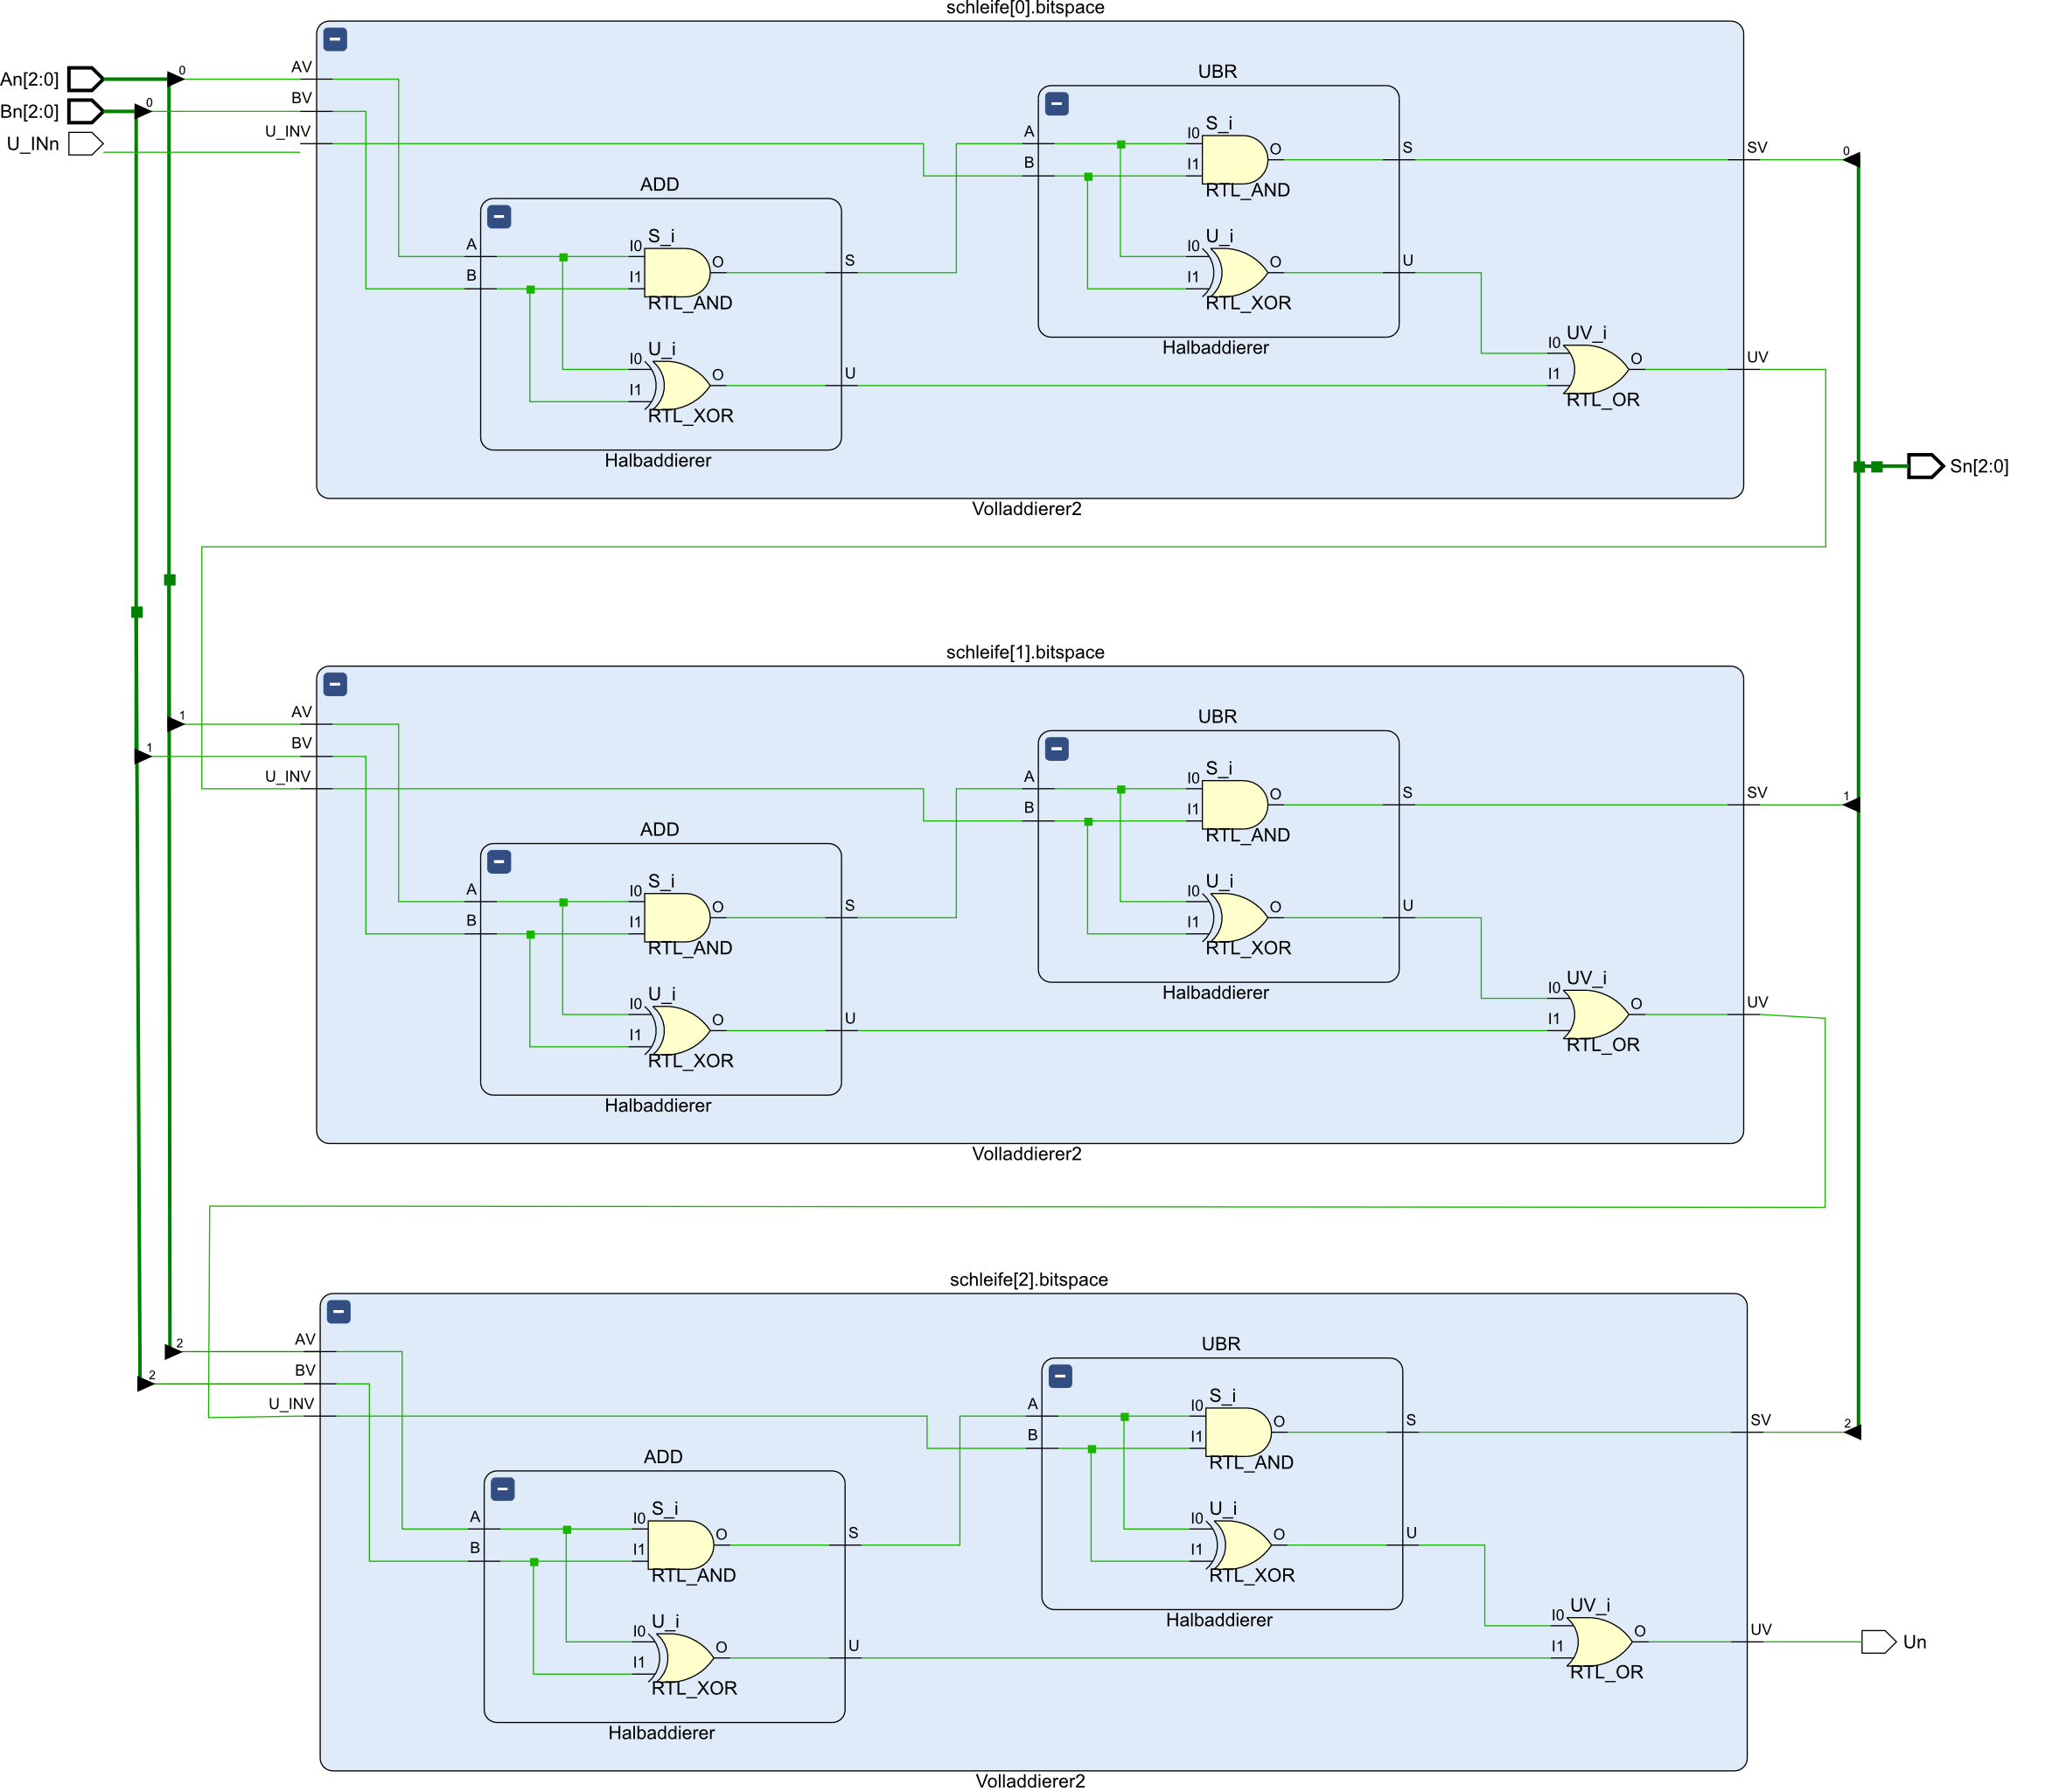
\includegraphics[width=\linewidth]{3bitaddierer.png}
				\caption{3-bit Addierers auf Basis von Volladdierern auf Gatterebene}
			\end{center}
		\end{figure}
	\subsection*{3.2}
		Für Gatterlaufzeit eines 4-bit-Addierers kann folgende berechnet werden.\\
		(Die folgende Beschreibung orientiert sich an der in 3.1 verwendeten Notation. Für ein XOR-Gatter wird ebenfalls 12 ns angenommen, trotz dessen das in einigen Architekturen das XOR-Gatter durch 3 Gatter realisiert wird.)\\
		Jeder Volladdierer kann parallel die ADD Halbaddierer berechnen(innerhalb dessen laufen die Gatter ebenfalls parallel ab), somit kostet das nur einmal 12 ns.\\
		Ferner kostet jeder UBR Halbaddierer (innerhalb dessen laufen die Gatter ebenfalls parallel ab) 12ns. Zu guter Letzt muss um den Eingangsübertag zu berechnen noch das OR-Gatter der Volladdierer berechnet werden. Es Resultiert die folgende Formel:
		\begin{equation}
			t(\text{bits}) = 12ns + 2\cdot 12ns\cdot \text{bits}
		\end{equation}
		Somit Resultiert für 4 bits eine Gatterlaufzeit von 108ns.
	\subsection*{3.3}
		$s = a + b$, wobei sich das Ergebnis s für die Addition von zwei 4-Bit Zahlen a,b sich wie gefolgt in Bitschreibweise zusammensetzt: $s = c_4 s_3s_2s_1s_0$ \\
		$s_i = a_i \oplus b_i \oplus c_i$ für $i \in \{0,1,2,3\}$ mit $c_0$ als $c_{in}$ und $c_4$ als letzten Übertrag \\
		\\
		$s_0 = a_0 \oplus b_0 \oplus c_0$ \\
		$s_1 = a_1 \oplus b_1 \oplus c_1$ \\
		$s_2 = a_2 \oplus b_2 \oplus c_2$ \\
		$s_3 = a_3 \oplus b_3 \oplus c_3$ \\
		$c_4$ \\
		\\
		\\
		Die Carries $c_i$ lassen mit den folgenden Schaltfunktionen vorberechnen \\
		$c_i = g_{i-1} \lor p_{i-1}c_{i-1}$ mit $g_i = a_ib_i$ und $p_i = a_i \lor b_i$, sodass \\
		\\
		$c_1 = g_0 \lor p_0c_0$  (Einmal ausführlich: $c_1 = a_0b_0 \lor (a_0 \lor b_0)c_0$)\\
		$c_2 = g_1 \lor p_1g_0 \lor p_1p_0c_0$ \\
		$c_3 = g_2 \lor p_2g_1 \lor p_2p_1g_0 \lor p_2p_1p_0c_0$ \\
		$c_4 = g_3 \lor p_3g_2 \lor p_3p_2g_1 \lor p_3p_2p_1g_0 \lor p_3p_2p_1p_0c_0$ \\
\end{document}
